% Options for packages loaded elsewhere
\PassOptionsToPackage{unicode}{hyperref}
\PassOptionsToPackage{hyphens}{url}
%
\documentclass[
  french,
]{article}
\usepackage{lmodern}
\usepackage{amssymb,amsmath}
\usepackage{ifxetex,ifluatex}
\ifnum 0\ifxetex 1\fi\ifluatex 1\fi=0 % if pdftex
  \usepackage[T1]{fontenc}
  \usepackage[utf8]{inputenc}
  \usepackage{textcomp} % provide euro and other symbols
\else % if luatex or xetex
  \usepackage{unicode-math}
  \defaultfontfeatures{Scale=MatchLowercase}
  \defaultfontfeatures[\rmfamily]{Ligatures=TeX,Scale=1}
\fi
% Use upquote if available, for straight quotes in verbatim environments
\IfFileExists{upquote.sty}{\usepackage{upquote}}{}
\IfFileExists{microtype.sty}{% use microtype if available
  \usepackage[]{microtype}
  \UseMicrotypeSet[protrusion]{basicmath} % disable protrusion for tt fonts
}{}
\makeatletter
\@ifundefined{KOMAClassName}{% if non-KOMA class
  \IfFileExists{parskip.sty}{%
    \usepackage{parskip}
  }{% else
    \setlength{\parindent}{0pt}
    \setlength{\parskip}{6pt plus 2pt minus 1pt}}
}{% if KOMA class
  \KOMAoptions{parskip=half}}
\makeatother
\usepackage{xcolor}
\IfFileExists{xurl.sty}{\usepackage{xurl}}{} % add URL line breaks if available
\IfFileExists{bookmark.sty}{\usepackage{bookmark}}{\usepackage{hyperref}}
\hypersetup{
  pdftitle={Synthèse des réponses au questionnaire relatifs aux ateliers du 5.10.20},
  pdfauthor={Nicolas Bressoud},
  pdflang={fr},
  hidelinks,
  pdfcreator={LaTeX via pandoc}}
\urlstyle{same} % disable monospaced font for URLs
\usepackage[margin=1in]{geometry}
\usepackage{longtable,booktabs}
% Correct order of tables after \paragraph or \subparagraph
\usepackage{etoolbox}
\makeatletter
\patchcmd\longtable{\par}{\if@noskipsec\mbox{}\fi\par}{}{}
\makeatother
% Allow footnotes in longtable head/foot
\IfFileExists{footnotehyper.sty}{\usepackage{footnotehyper}}{\usepackage{footnote}}
\makesavenoteenv{longtable}
\usepackage{graphicx}
\makeatletter
\def\maxwidth{\ifdim\Gin@nat@width>\linewidth\linewidth\else\Gin@nat@width\fi}
\def\maxheight{\ifdim\Gin@nat@height>\textheight\textheight\else\Gin@nat@height\fi}
\makeatother
% Scale images if necessary, so that they will not overflow the page
% margins by default, and it is still possible to overwrite the defaults
% using explicit options in \includegraphics[width, height, ...]{}
\setkeys{Gin}{width=\maxwidth,height=\maxheight,keepaspectratio}
% Set default figure placement to htbp
\makeatletter
\def\fps@figure{htbp}
\makeatother
\setlength{\emergencystretch}{3em} % prevent overfull lines
\providecommand{\tightlist}{%
  \setlength{\itemsep}{0pt}\setlength{\parskip}{0pt}}
\setcounter{secnumdepth}{5}
\ifxetex
  % Load polyglossia as late as possible: uses bidi with RTL langages (e.g. Hebrew, Arabic)
  \usepackage{polyglossia}
  \setmainlanguage[]{french}
\else
  \usepackage[shorthands=off,main=french]{babel}
\fi

\title{Synthèse des réponses au questionnaire relatifs aux ateliers du 5.10.20}
\author{Nicolas Bressoud}
\date{novembre 2020}

\begin{document}
\maketitle

\renewcommand*\contentsname{Table des matières}
{
\setcounter{tocdepth}{2}
\tableofcontents
}
\hypertarget{contexte}{%
\section{Contexte}\label{contexte}}

Ce rapport concerne les résultats bruts liés à l'évaluation, par les personnels, des workshops du 5 octobre 2020.

\hypertarget{donnuxe9es-de-base}{%
\section{Données de base}\label{donnuxe9es-de-base}}

Nombres de personnes qui ont reçu les informations sur les workshops : 148

Nombre de personnes inscrites aux ateliers : 75 / 148

Nombres de participant·es au questionnaire : 27 / 148

Résumé des origines des participant·es (langue, catégories) :

\begin{table}

\caption{\label{tab:table}résumé de l'échantillon}
\centering
\begin{tabular}[t]{l|l|r}
\hline
lan & cat & n\\
\hline
Deutsch & profs & 7\\
\hline
Deutsch & direction élargie & 2\\
\hline
Deutsch & animation & 1\\
\hline
Français & profs & 10\\
\hline
Français & direction élargie & 3\\
\hline
Français & animation & 1\\
\hline
Français & admin et secrétariat & 3\\
\hline
\end{tabular}
\end{table}

\hypertarget{plots}{%
\section{Plots}\label{plots}}

\hypertarget{par-site}{%
\subsection{Par site}\label{par-site}}

Les graphiques suivants présentent les résumés de chaque item par langue.

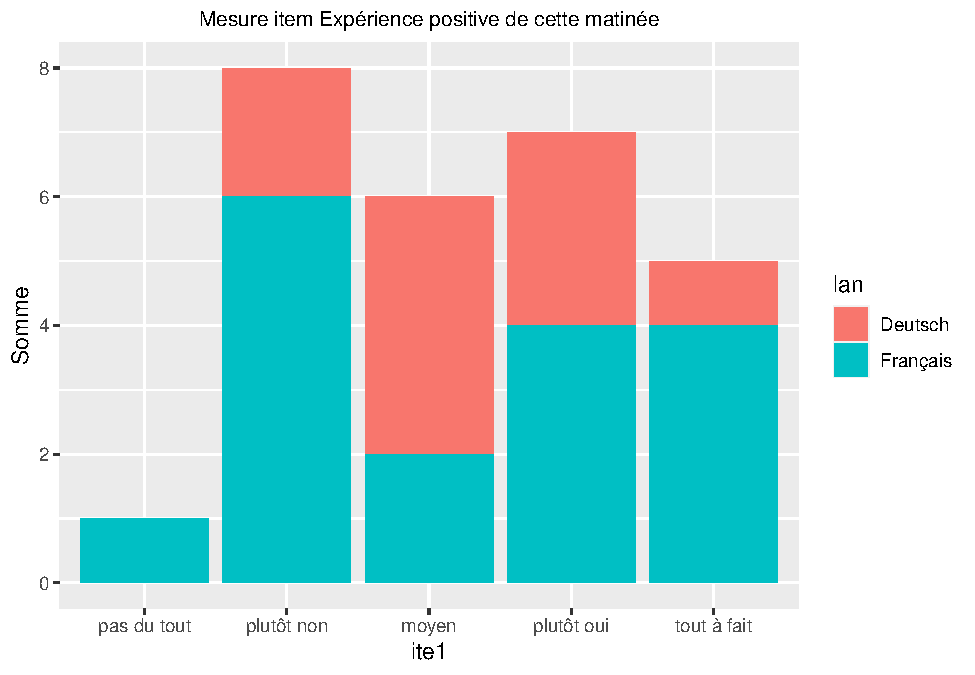
\includegraphics[width=0.5\linewidth]{hepvs2020_nb_rapport_files/figure-latex/vis-1} 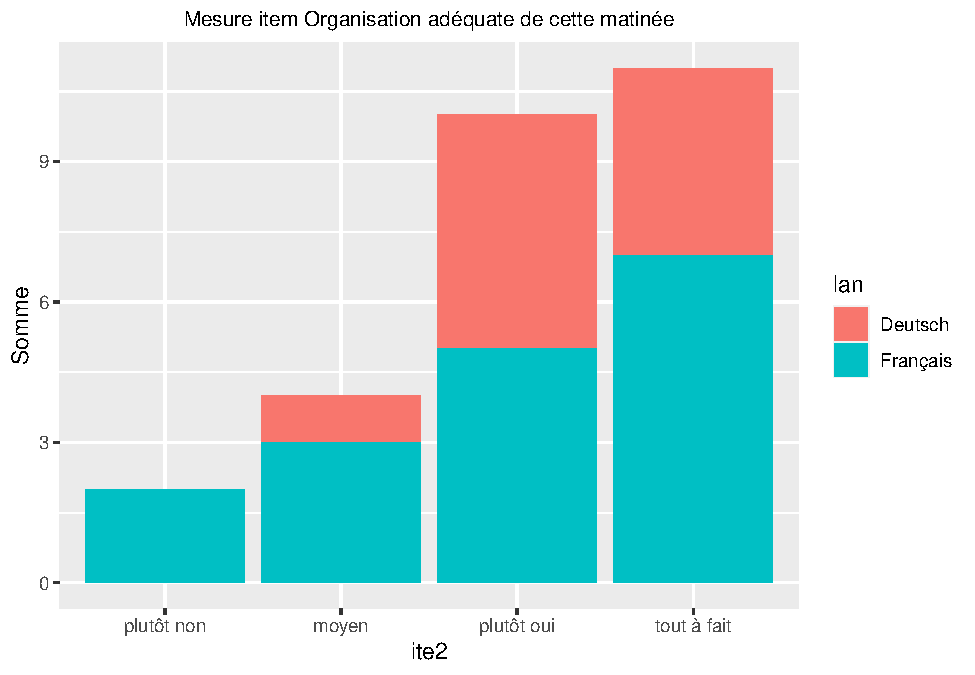
\includegraphics[width=0.5\linewidth]{hepvs2020_nb_rapport_files/figure-latex/vis-2} 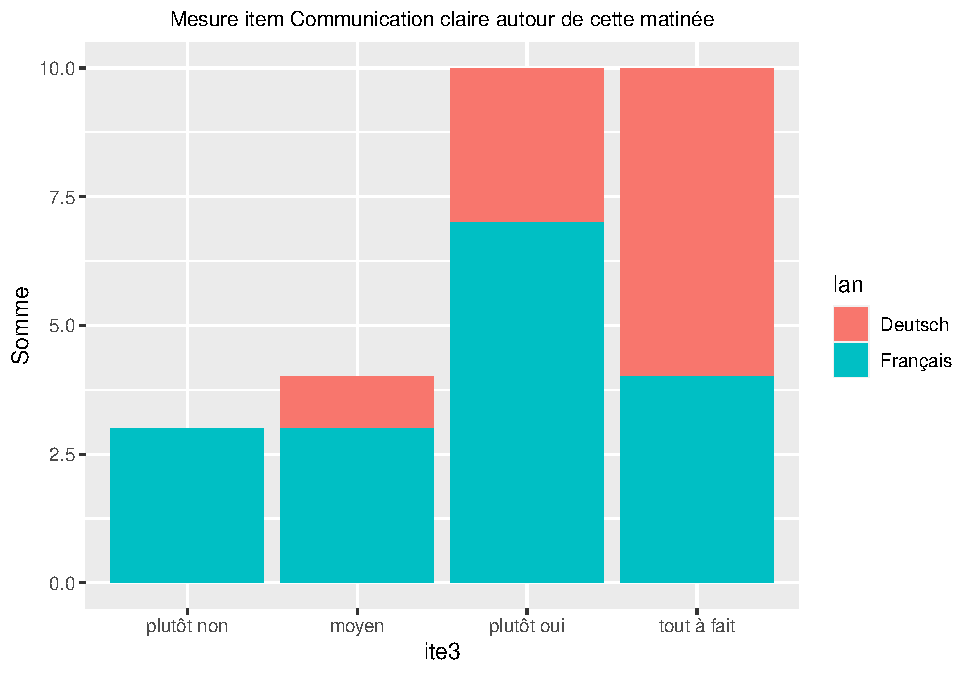
\includegraphics[width=0.5\linewidth]{hepvs2020_nb_rapport_files/figure-latex/vis-3} 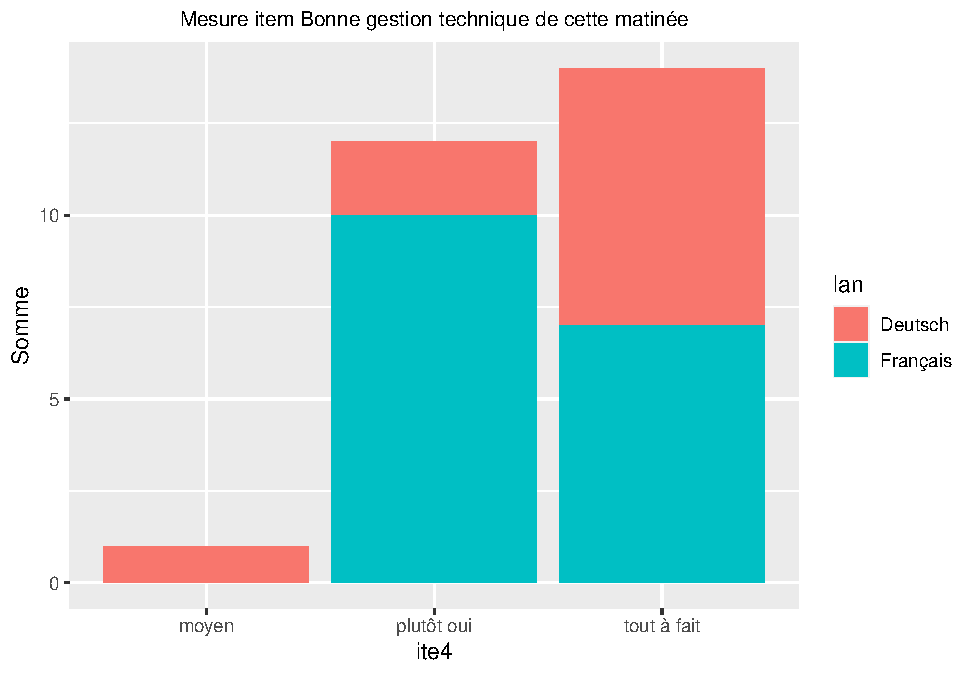
\includegraphics[width=0.5\linewidth]{hepvs2020_nb_rapport_files/figure-latex/vis-4} 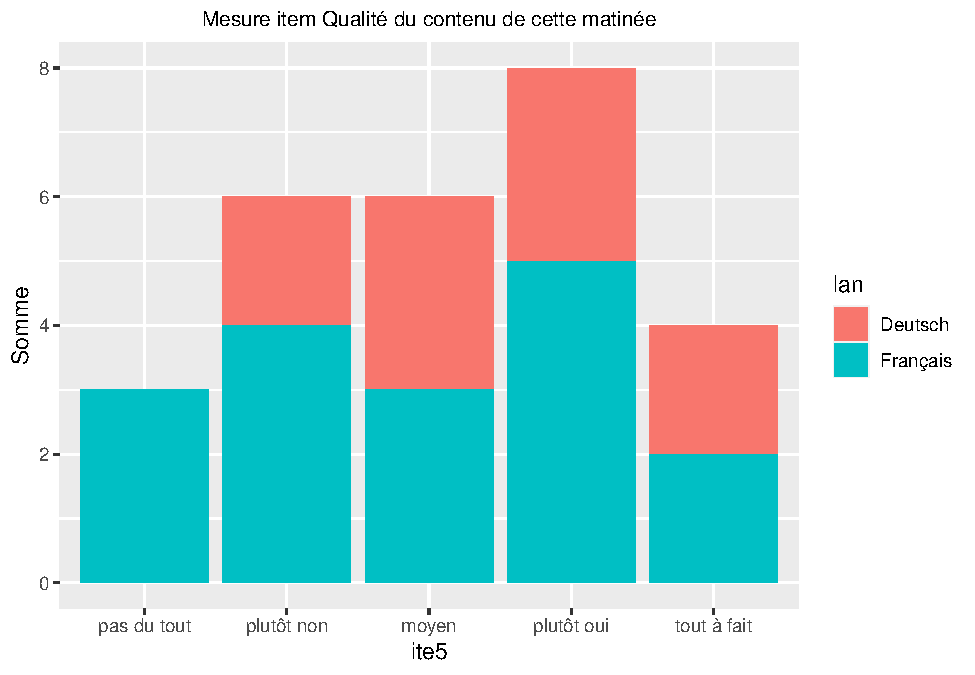
\includegraphics[width=0.5\linewidth]{hepvs2020_nb_rapport_files/figure-latex/vis-5} 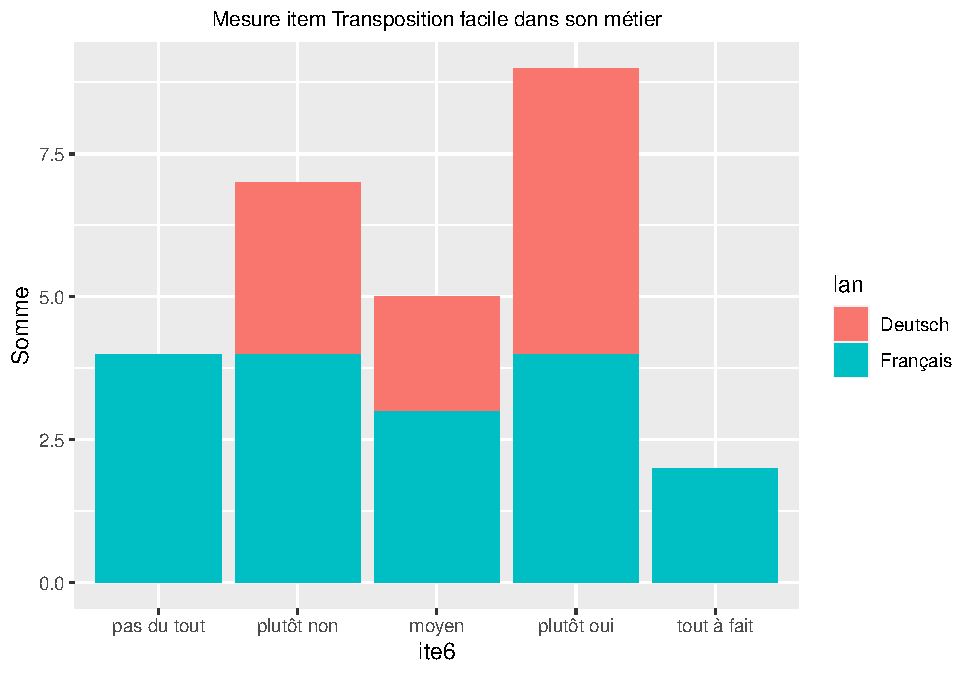
\includegraphics[width=0.5\linewidth]{hepvs2020_nb_rapport_files/figure-latex/vis-6} 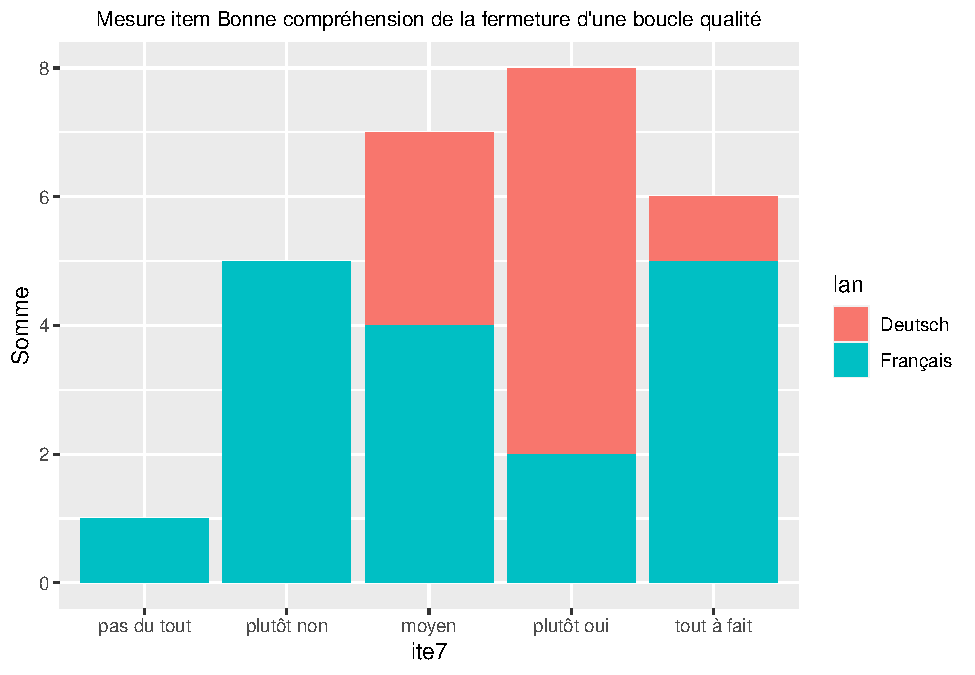
\includegraphics[width=0.5\linewidth]{hepvs2020_nb_rapport_files/figure-latex/vis-7} 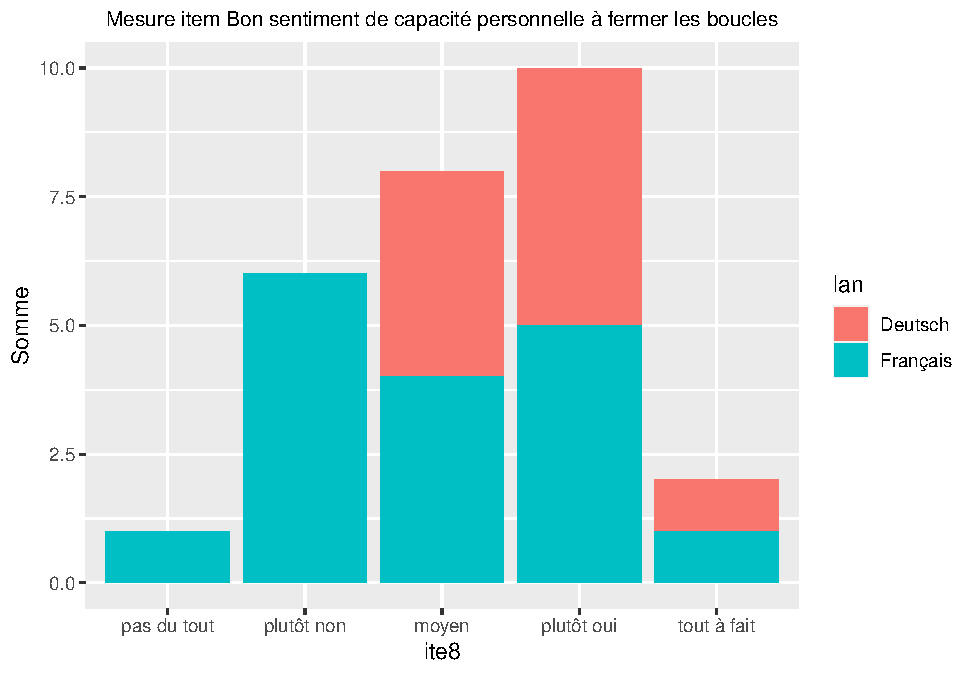
\includegraphics[width=0.5\linewidth]{hepvs2020_nb_rapport_files/figure-latex/vis-8}

\hypertarget{par-catuxe9gorie-de-personnels}{%
\subsection{Par catégorie de personnels}\label{par-catuxe9gorie-de-personnels}}

Les graphiques suivants présentent les résumés de chaque item par catégorie de personnels

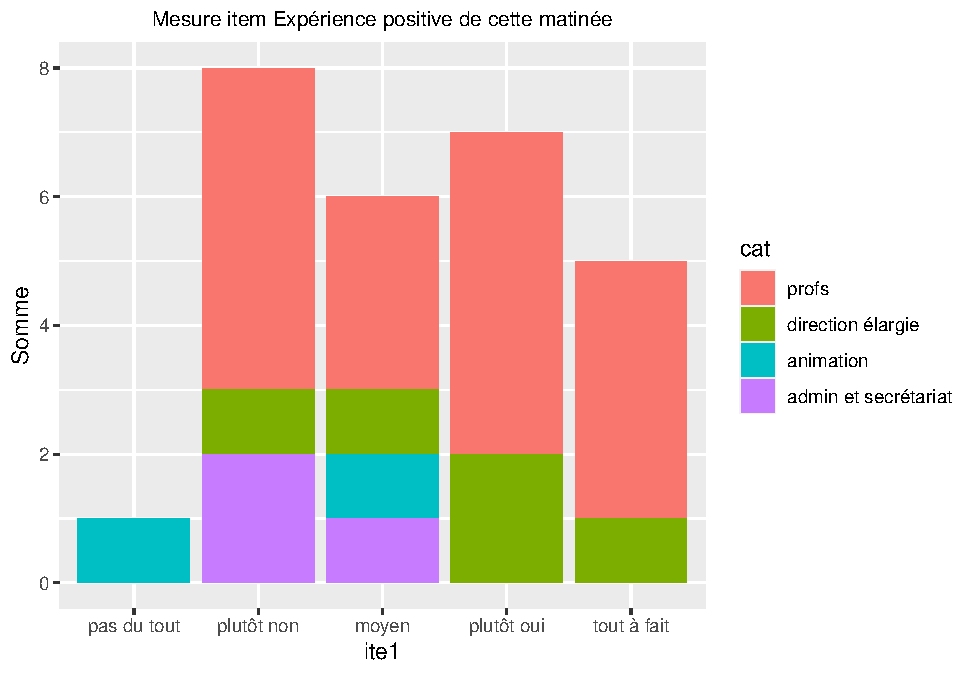
\includegraphics[width=0.5\linewidth]{hepvs2020_nb_rapport_files/figure-latex/vis2-1} 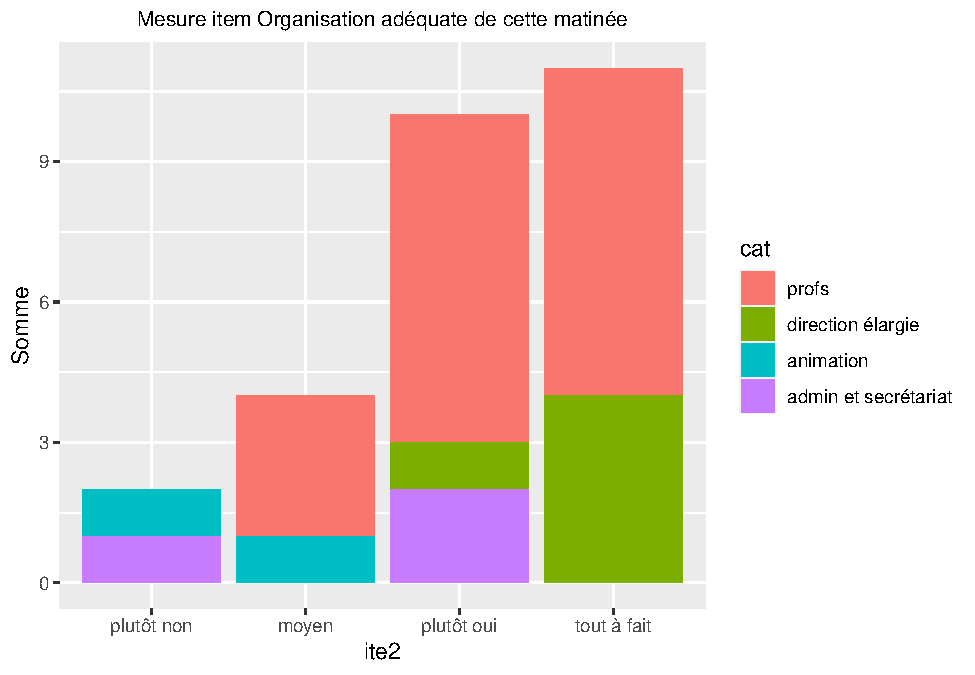
\includegraphics[width=0.5\linewidth]{hepvs2020_nb_rapport_files/figure-latex/vis2-2} 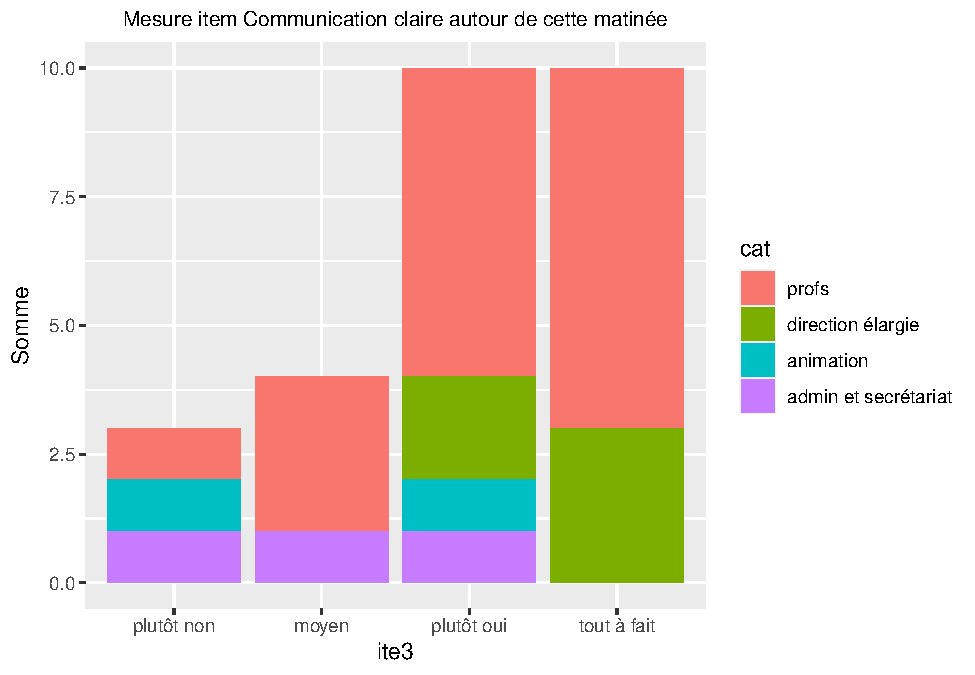
\includegraphics[width=0.5\linewidth]{hepvs2020_nb_rapport_files/figure-latex/vis2-3} 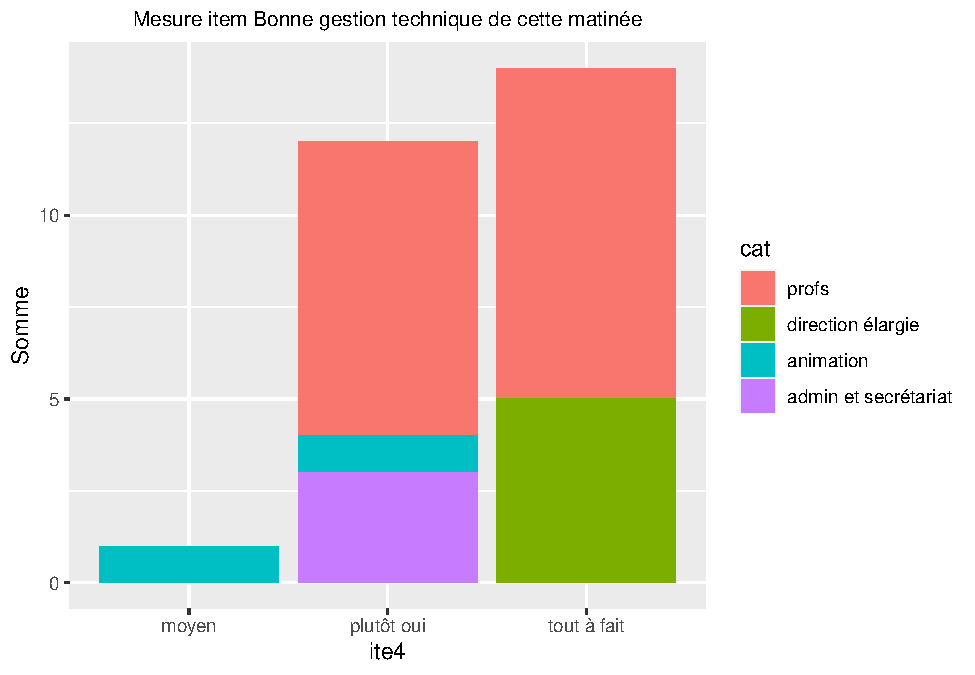
\includegraphics[width=0.5\linewidth]{hepvs2020_nb_rapport_files/figure-latex/vis2-4} 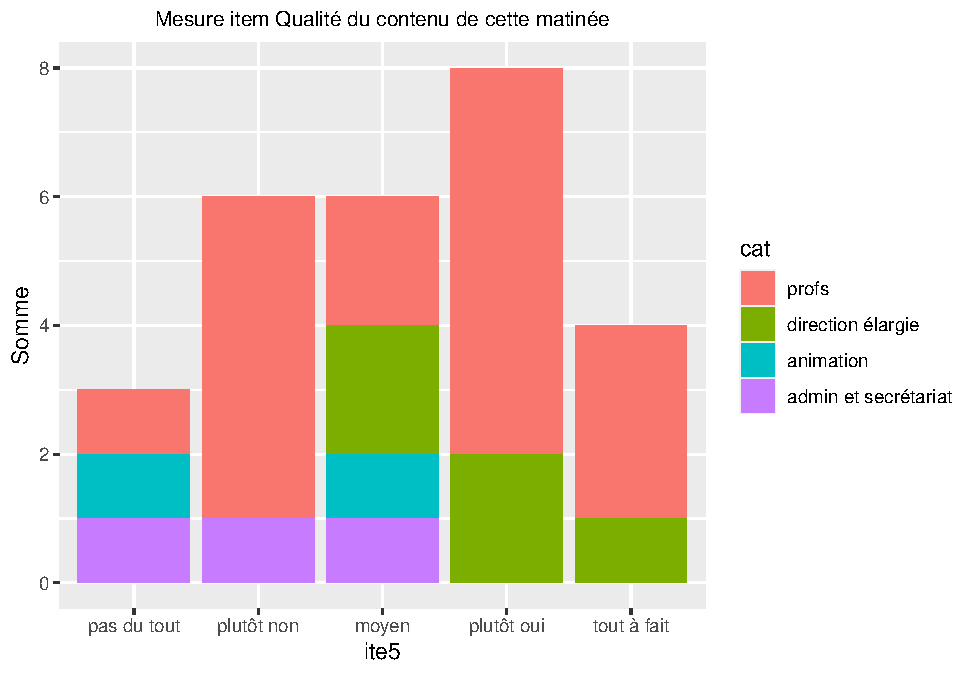
\includegraphics[width=0.5\linewidth]{hepvs2020_nb_rapport_files/figure-latex/vis2-5} 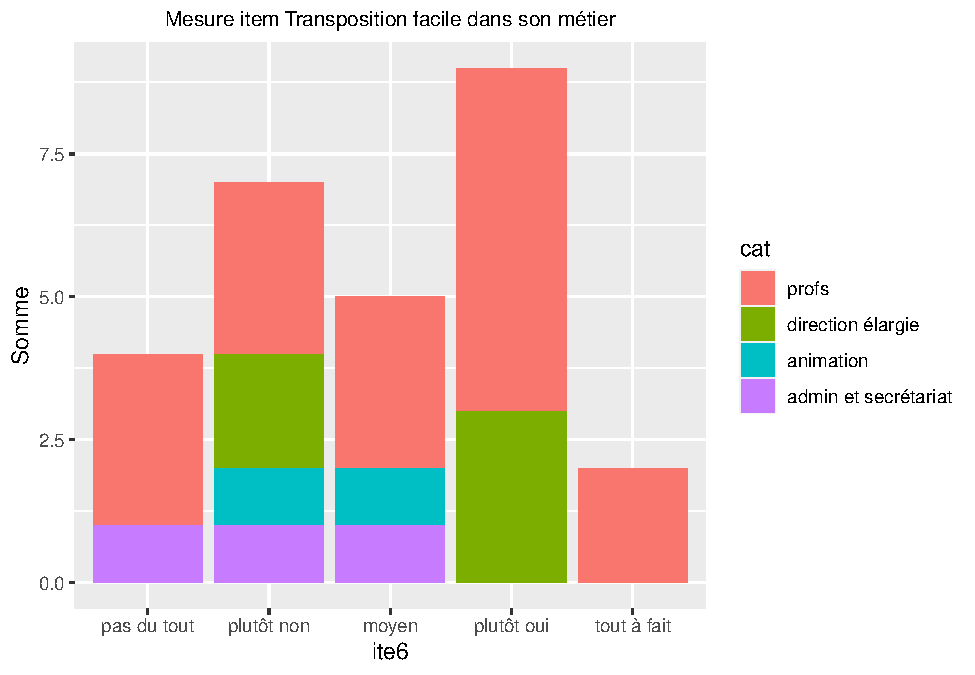
\includegraphics[width=0.5\linewidth]{hepvs2020_nb_rapport_files/figure-latex/vis2-6} 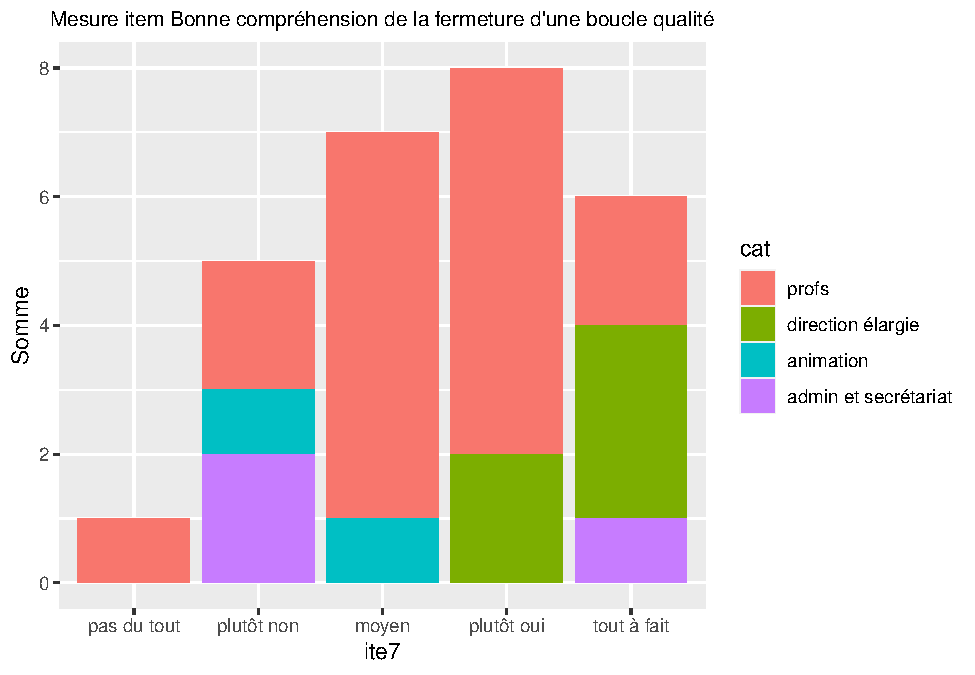
\includegraphics[width=0.5\linewidth]{hepvs2020_nb_rapport_files/figure-latex/vis2-7} 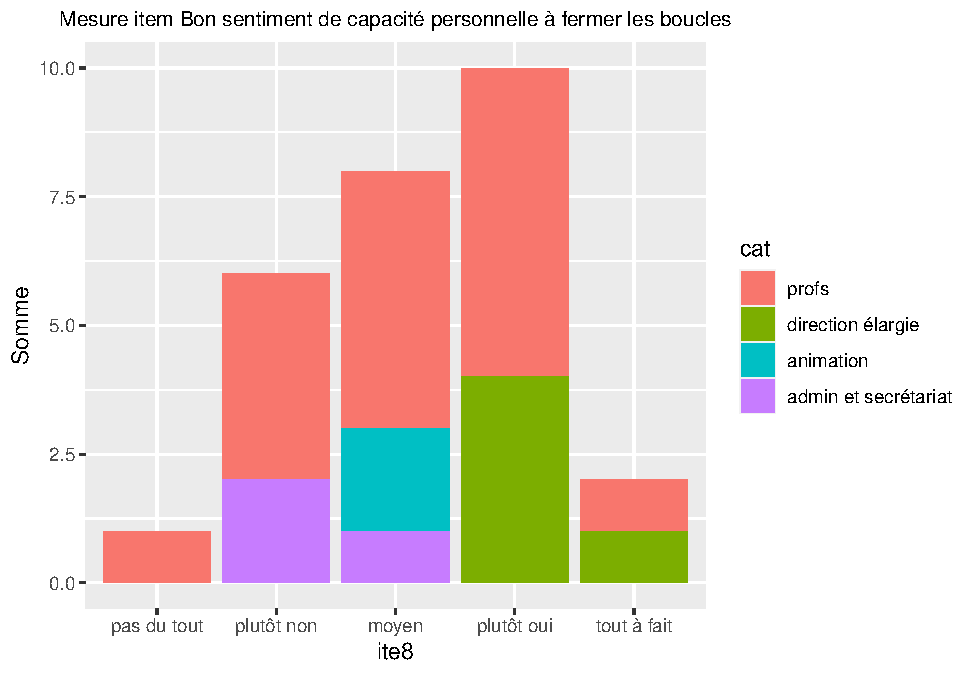
\includegraphics[width=0.5\linewidth]{hepvs2020_nb_rapport_files/figure-latex/vis2-8}

\hypertarget{retours-qualitatifs}{%
\section{Retours qualitatifs}\label{retours-qualitatifs}}

\hypertarget{item-1}{%
\subsection{Item 1}\label{item-1}}

Pouvez-vous formuler ici vos besoins en matière d'accompagnement pour votre développement professionnel ? / Können Sie hier Ihre Bedürfnisse in Bezug auf die Unterstützung Ihrer beruflichen Entwicklung formulieren?

\begin{itemize}
\tightlist
\item
  Es wäre schön wieder einmal ein Mitarbeitergespräch mit den Vorgesetzten eingeladen zu werden. Mein letztes offizielles MAG war vor 10 Jahren und meine letzte Anfrage dies betreffend ist seit 10 Monaten unbeantwortet.
\item
  Mich mehr einbringen können ins Evasys, weil ich dann mehr herausholen könnte.
\item
  Sobald das Portfolio zur Verfügung steht, wäre ich froh um eine Einführung.
\item
  weitere Angebote während dem Studienjahr, um die Mitarbeitenden in der Schliessung ihrer Qualitätskreisläufe zu schliessen.
\item
  Regelmässige solche Workshops wie am 5.10 finde ich im Prinzip sinnvoll. Sie erinnern mich an die Prozesse und erhöhen meine Motivation.
\item
  Forschung und Lehre
\item
  Ich könnte die Inhalte mit 2-3 kurzen Stichpunkten besser verinnerlichen und verwirklichen.
\item
  Habe im Moment keine Bedürfnisse.
  Ich freue mich auf die CAS Fachberatung-Ausbildung. Ich sehe dies als Unterstützung in meiner beruflichen Entwicklung als Fachberatung.
\item
  ``Principal besoin: prendre le temps pour le faire (et avoir ce temps), voir que j'ai prise sur le début de la boucle afin d'être motivé à aller jusqu'au bout.''
\item
  pas de besoin particulier
\item
  "Je ne saurais répondre à cette question tellement l'accompagnement pour mon développement professionnel a été inexistant depuis mon insertion au sein de la HEP. Je dis bien l'accompagnement et non des discussions, car il y en a eues.
\item
  Jusqu'à présent, les quelques discussions que j'ai eues avec des responsables à ce sujet étaient conduites dans une vision manichéenne.
  Les besoins touchent donc concrètement à une manière de faire et d'accompagner, mais aussi aux attentes et à ce que signifie l'apprentissage pour la vie. "
\item
  à ce stade dans mon domaine les choses sont claires et bien dirigées
\item
  Pour le moment, aucun besoin
\item
  Le/la/les responsables RH/administration devraient connaître les compétences du personnel, leur attribuer un poste ou des tâches en fonction et non répartir le travail de façon indistincte. Un développement professionnel ou une formation continue aurait ensuite du sens.
\item
  Moins de superficialité, de cosmétique, d'alibi. Un vrai regard sur les pratiques de cette institution, en profondeur, pour espérer toucher aux véritables difficultés et dysfonctionnements et espérer les améliorer.
\item
  Il me semble que ce qui me manquerait essentiellement, c'est un ``esprit de corps'' ou une ``philosophie d'entreprise'' claire. On ne cesse de courir après le temps pour remplir nos missions et les moment conviviaux, de réseautage et d'échanges d'expérience manquent. Cette période est peut-être une bonne occasion pour créer plus de cohésion.
\item
  Je trouve les entretiens d'appréciation très pertinents. Ils m'apportent énormément pour mon développement professionnel, donc à maintenir pour ma part, à mettre en place pour mes collègues.
\item
  Pour l'instant, aucun.
\item
  "Je n'aurais aucune envie d'avoir un accompagnement par le soutien à l'enseignement et à l'apprentissage dont les compétences en termes de pédagogie et de didactique et dans mon champ d'enseignement ne me paraissent pas en lien.
\item
  Je souhaiterais par contre pouvoir analyser les évaluations evasys avec un membre du groupe qualité.
\item
  Je mettrais également en avant l'intérêt de partager avec des collègues (style communauté de pratique) sur l'analyse des évaluations evasys et des retours et régulations proposées.
\item
  De manière très direct, qu'est-ce qui est attendu de moi par rapport à la qualité à la HEPVS.
\item
  A ce jour, je n'ai bénéficié d'aucun accompagnement spécifique pour mon développement professionnel spécifique. J'ai suivi les différentes ``sensibilisations'' au sein de l'institution. Je me suis débrouillé au travers des différentes formations externes. Il manque un véritable service de gestion des ressources humaines qui permette aux personnels de faire part de leurs besoins, de répondre aux besoins de l'institution. Tout est à créé !
\item
  Reconnaissance des équipes disciplinaires et des coordinateurs ; ressources administratives et techniques à disposition des équipes pour archivage et complétion des boucles qualités
\end{itemize}

\hypertarget{item-2}{%
\subsection{Item 2}\label{item-2}}

Vous pouvez laisser ici un commentaire pour préciser l'un ou l'autre aspect de cette matinée du 5 octobre. / Sie können hier einen Kommentar hinterlassen, um jeden Aspekt des Vormittags des 5. Oktober zu klären.

\begin{itemize}
\tightlist
\item
  Ich verstehe dieses Frage nicht.
\item
  Der Workshop hat einen interessanten Einblick in das Instrument Portfolio gegeben - ich hoffe, baldmöglichst ein solches Instrument zur persönlichen und beruflichen Weiterentwicklung zur Verfügung zu haben.
  Vielen Dank für das tolle Angebot!
\item
  Ich habe einen guten Überblick erhalten.
\item
  Danke für euer Engagement.
\item
  Leider konnte ich nicht am Workshop teilnehmen, da ich am Vormittag des 5.Oktober an der Orientierungsschule unterrichtete.
\item
  J'étais dans l'atelier sur les entretiens de collaboration et nous avons eu de bons échanges.
\item
  ``L'atelier auquel je participais, a dévié sur une thématique''``syndicale''``, en s'éloignant du sujet. Les objectifs n'ont peut-être pas été assez clairement édictés, ils n'ont pas été rappelés en cours de workshop, une partie des participants (les principaux''``contributeurs''``) adoptant par ailleurs une position de non entrée en matière sur la thématique, l'atelier a eu peu d'utilité, voire à contribué à soulever des problèmes plus que donner des pistes de solutions. De plus, je pensais qu'on allait nous présenter des outils en cours de développement et vérifier s'ils correspondaient aux besoins\ldots{} alors qu'en fait on demandait au participants quels outils leurs seraient utiles dans le domaine de la qualité. Question trop large pour pouvoir contribuer efficacement.''
\item
  il est difficile de faire rentrer certains dans le processus qualité, l'individu laissant alors peu de place à l'institution
\item
  Il aurait peut-être fallu un atelier que pour le service administratif
\item
  Cette rencontre et discussion a, malheureusement, été noyée dans le trop plein d'informations que nous recevons dans notre métier (mails, réunions\ldots). L'idée de précéder les rencontres par des vidéos est très chouette. Néanmoins elles étaient basées sur des théories et il manquait, selon moi, des canevas clairs sur ce qui était attendu de nous pendant la discussion. Que devons-nous changer, qui va le faire, comment, lister les moyens\ldots{} tout selon manquait fâcheusement! Un message clair dès le départ est primordial pour motiver les troupes.
\item
  Sans une information préalable sur les termes ``boucle de qualité'' et ``management des idées'' il n'était pas possible de prendre part à la discussion. Difficile également de participer à un atelier mi-PAT, mi-enseignement. Par contre, vu le nombre d'inscrits, heureusement que la parole n'a été monopolisée que par 4 ou 5 personnes !
\item
  Déception, incompréhension, alibi\ldots{}
\item
  Honnêtement, je n'ai pas vraiment compris l'objectif de l'atelier et les retombées concrètes qu'il pourrait avoir.
\item
  Workshop très difficile à comprendre pour le groupe dans lequel j'étais. Monopolisation de la parole par certains. Seules 4 personnes se sont exprimées pour se plaindre principalement. Beaucoup de commentaires n'étaient pas en lien avec les questions préalablement proposées. Peu de solutions constructives proposées. Mais c'est mon impression. Bravo aux rédacteur / rédactrice de la synthèse du groupe d'avoir réussi à retranscrire les idées sous-jacentes que je n'ai pas perçues dans les plaintes incessantes. Personnellement, je n'ai pas apprécié cette matinée, pas du point de vue de l'organisation, de la gestion de l'équipe qualité et tout, mais du point de vue de certains collègues et de leur attitude. Merci à toute l'équipe qualité pour le travail titanesque qu'elle effectue!
\item
  La notion de ``café-croissant virtuel'' (ou expression analogue) n'est pas forcément convaincante\ldots{} De mon point de vue une seule connexion aux ateliers aurait suffi.
\item
  "Je trouve important d'informer les étudiants du cadre éthique de ces évaluations et de la suppression de toute évaluation inadéquate.
\item
  J'ai bcp apprécié ces échanges et constaté l'intérêt d'en parler alors que souvent ces choses ne sont pas dites par peur du jugement.
\item
  J'ai particulièrement apprécié la finesse de la conduite des interactions dans cet atelier et la mise en confiance ainsi générée.
\item
  Bravo et merci
\item
  Beaucoup d'énergie mise au niveau de la forme. Un temps fou a sans doute dû être consacrée par l'équipe organisatrice qui s'est donnée pour préparer ce moment. Par contre au niveau du contenu, toujours la même chose: des discussions de groupe, puis\ldots rien\ldots pour en faire quoi? Pour avoir discuté avec des collègues, la qualité des différents groupes était fort différente et dépendait (évidemment) de la qualité de préparation de l'animateur. Dans mon groupe, nous avons dû nous prononcer sur un document dont nous n'avions pas pu prendre connaissance à l'avance. On ne savait pas trop de quoi il en retournait. La discussion a été à bâton rompu. Je ne vois pas sur quoi cela peut déboucher. Je suis très déçue, d'autant que j'attendais bcp de ce ``renouveau'' au sein du groupe qualité. Je m'excuse de ce propos sévère, mais nous sommes toujours déconnectés des réels besoins du personnel et de l'institution, pour satisfaire à des labels ou des exigences externes\ldots{} dommage, il y aurait tant à faire dans notre école.
\end{itemize}

\end{document}
